\documentclass[11pt,a4paper,twoside,titlepage,british]{report}
\setlength{\topmargin}{18pt}
\usepackage{layout}
\usepackage[utf8]{inputenc}         % special chars
\usepackage[babel]{csquotes}        % context-sensitive quotation
\usepackage[dvipsnames]{xcolor}     % some predefined colors
\usepackage[plain]{fancyref}        % provides \fref and \Fref for referencing
\usepackage[T1]{fontenc}
\usepackage{babel}
\usepackage{isodate}
\usepackage{fancyhdr}
\usepackage{geometry}
\usepackage{hyperref}
\usepackage[style=numeric-comp,sorting=none,backend=biber]{biblatex}
\usepackage{graphicx}
\usepackage{setspace}
\usepackage{amsmath}
\usepackage{float}
\usepackage{listings}
\usepackage{caption}
\usepackage{svg}
\usepackage{algorithm}
\usepackage{algorithmic}
\usepackage{amsthm}

\theoremstyle{definition}
\newtheorem{definition}{Definition}[section]

\geometry{
    textheight=595pt,
    textwidth=360pt,
}

\addbibresource{main.bib}
\nocite{*}

%=======================================================================================================================

\fancyhf{}
\fancyfoot[LE,RO]{\thepage}
\fancyhead[LE,RO]{\slshape \nouppercase{\leftmark}}
\renewcommand*{\headrulewidth}{0pt}
\renewcommand*{\footrulewidth}{0pt}
\fancypagestyle{plain}{%
  \fancyhf{}
  \fancyfoot[LE,RO]{\thepage}
}
\renewcommand*{\chaptermark}[1]{\markboth{\thechapter.\ #1}{}}
\renewcommand*{\sectionmark}[1]{\markright{\thesection.\ #1}}

%=======================================================================================================================

\author{Lukas Wilde}
\date{31.08.2022}
\title{Workload-based Data Partitioning for Index Construction}

%=======================================================================================================================

\makeatletter
\let\runauthor\@author
\let\runtitle\@title
\let\rundate\@date
\makeatother
\sloppy

%=======================================================================================================================

\begin{document}
\pagenumbering{roman}
\begin{titlepage}
    \begin{center}
        \includegraphics[scale=.5]{figures/logo.pdf}

        \bfseries
        \vspace{2em}
        Faculty of Mathematics and Computer Science \\
        Department of Computer Science

        \vspace{2cm}
        \begin{doublespace}
            {\LARGE \runtitle}
        \end{doublespace}

        \vspace{1cm} 
        {\large Bachelor's Thesis}

        \vfill
        {\normalfont written by}
        \\[1em]
        {\Large \runauthor}
        \\[1em]
        \textbf{\printdate{\rundate}}

        \vfill
        {\normalfont Supervisor}
        \\
        {\large Prof.~Dr.~Jens~Dittrich}
        \\[.5em]
        {\normalfont Advisors}
        \\
        {\large Joris~Nix}
        \\
        {\large Christian~Schön}
        \\[.5em]
        {\normalfont 1st Reviewer}
        \\
        {\large Prof.~Dr.~Jens~Dittrich}
        \\[.5em]
        {\normalfont 2nd Reviewer}
        \\
        {\large Prof.~Dr.~Felix~Schuhknecht}
    \end{center}
\end{titlepage}
\setcounter{page}{2}

%=======================================================================================================================

\cleardoublepage
\thispagestyle{plain}
\vspace*{\fill}

\subsection*{Eidesstattliche Erklärung}
Ich erkläre hiermit an Eides Statt, dass ich die vorliegende Arbeit selbstständig verfasst und keine anderen als die
angegebenen Quellen und Hilfsmittel verwendet habe.

\subsection*{Statement in Lieu of an Oath}
I hereby confirm that I have written this thesis on my own and that I have not used any other media or materials than
the ones referred to in this thesis.

\vspace{2cm}

\subsection*{Einverständniserklärung}
Ich bin damit einverstanden, dass meine (bestandene) Arbeit in beiden Versionen in die Bibliothek der Informatik
aufgenommen und damit veröffentlicht wird.

\subsection*{Declaration of Consent}
I agree to make both versions of my thesis (with a passing grade) acessible to the public by having them added to the
library of the Computer Science Department.

\vspace{2.5cm}

\begin{tabular}{ c c c c }
    Saarbrücken, & \makebox[4cm]{\hrulefill} & & \makebox[4cm]{\hrulefill} \\ [-2.2mm] 
               & \tiny Datum/Date                &              & \tiny Unterschrift/Signature \\
\end{tabular}

\vspace*{\fill}


%=======================================================================================================================

\input{0-2-acknowledgement.tex}
\clearpage
\thispagestyle{plain}

\chapter*{Abstract}
Database Management Systems routinely use index structures to improve lookup performance compared to simple scans. Many recent index structures use the underlying data distribution to apply optimizations. What only a few do is also incorporate workload information. For this reason, we design two partitioning algorithms that utilize a workload sample to create meaningful partitions, which can be used as the leaf nodes of a customizable index. We evaluate the lookup times for different query workloads on such an index and compare it to state-of-the-art index structures. The two workload properties that we investigate are \textit{frequency} and \textit{query type} of individual data points. We found that when partitioning for query type purity, the resulting index can easily change its data structures according to the query type in one partition. Such changes can result in an improvement of the average lookup time from 350 ns to 250 ns. For the frequency partitioning, we found that without optimizing the index to incorporate frequency information, it is not competitive with the state-of-the-art. However, we also found that the lookup performance was comparable to a B-tree even in the worst case.

%=======================================================================================================================

\cleardoublepage
\thispagestyle{plain}
\setcounter{tocdepth}{1} % do not print subsections
\setcounter{tocdepth}{2} % but add them to the PDF
\tableofcontents

\listoffigures
\listoftables

%=======================================================================================================================

\cleardoublepage
\pagenumbering{arabic}
\chapter{Introduction}
Over the years, a plethora of index structures have been proposed to deal with emerging difficulties and opportunities like cache efficiency or main-memory design. Designing a new index takes time and maybe covers only specific situations, which is why we have seen a recent attempt to abandon handcrafted indexes altogether. The approach by \citeauthor{Dittrich2021} \cite{Dittrich2021} uses genetic search with an initial population of generalized index structures to breed new and better indexes. Bred indexes are then evaluated using a fitness function over some workload. Since the leaf nodes of the indexes in their framework do not have a fixed size, we can fill them with whatever amount of data we feel is suitable. In our opinion, a good starting index would already incorporate the workload information on which it will later be evaluated. However, it is not clear what information about the workload could be used to create a good starting index. 

In the indexing world, we know that certain types of indexes are better for certain scenarios than others. For example, a B-tree with ISAM is a good choice for range queries, whereas a hash table delivers the best performance for point queries. Therefore, it would be beneficial to have the index leaves as individual parts that can change their data structure based on the queries. Apart from this, we also know that the nodes in the upper layers of a B-tree are usually cached when executing a workload because they are traversed for most queries. The logical consequence for our index would be placing leaves requested very often higher up in the index. The two relevant workload properties for these two cases are the \textit{query type purity} and the \textit{frequency} inside a leaf.

In our work, we aim to develop two partitioning algorithms that analyze the workload and use these two properties to create suitable partitions of our data. These partitions could then be used as the leaves of an index, where they are also mutated as described above. We use different workloads to evaluate the partitioning algorithms and compare the resulting index against the state-of-the-art. 

\clearpage
\noindent The rest of this thesis is structured in the following way. We first provide an overview of related work in \Cref{sec:related_work}. Most of it introduces different index structures that we will either use as comparison points in benchmarks or that apply some sort of partitioning to the data.

\noindent Afterwards, we look at the necessary background needed to understand our partitioning algorithms in \Cref{sec:background}. This includes what we define as partitions and how they can be applied to the indexing domain. We also introduce the indexing framework that we used to evaluate our partitioning algorithms and present how one can approximate the first-order derivative of discrete functions. 

\noindent \Cref{sec:framework} showcases the design of our partitioning algorithms and the framework we used to evaluate them. We go over each step in the pipeline to understand the methods that are applied in our evaluation.

\noindent This evaluation is then covered in \Cref{sec:evaluation} where we present the experimental setup, get a deeper understanding of how the partitioning algorithms work, and eventually report the results of the experiments we conducted.

\noindent The results are then summarized in \Cref{sec:conclusion}, and we present possible directions for further research in this area.



%=======================================================================================================================

\clearpage
\thispagestyle{plain}
\chapter{Related Work}\label{sec:related_work}

In this Chapter, we first introduce the index structures that served as a baseline to compare our algorithms. We cover traditional tree-like index structures like the B$^+$-tree, look into Radix Trees represented by the Adaptive Radix Tree and then proceed to Learned index structures like the Recursive Model Index and the Piecewise Geometric Index. After that, we explore two fields in which the query workload is used in data partitioning: Adaptive Hybrid Indexes and Distributed Database Systems.

\paragraph{} 
When we look at traditional tree-like index structures, the well-known B$^+$-tree \cite{Bayer1970-rh} is the first index that comes to mind. It was designed to index a dynamically changing file with the assumption that only a small part of the index can remain in main memory at all times. The authors acknowledged that this file can be subject to change, and as such one would need efficient ways to not only search the index, but also enable the insertion and deletion of existing keys. The nodes in a B$^+$-tree are always containing at least $k$ and at most $2k$ keys at a time, resulting in a space occupancy of at least 50\%. The keys in inner nodes act as boundaries to guide the retrieval, essentially producing disjoint ranges. Should a key fall into a specific range, the corresponding child pointer is used to get to the node of the next layer. The keys in the nodes are ordered, which allows for an efficient binary search. Insertion and deletion follow the same principle, except when inserting or deleting a key would result in a key count of less than $k$ or more than $2k$ inside a node. In this case, neighboring nodes need to be merged or a node needs to be split in order to guarantee the invariant that each node contains between $k$ and $2k$ keys. The advantage of this sort of index is that the keys are kept ordered, which enables efficient predecessor/successor queries and range queries. However, B$^+$-trees have a poor cache utilization, since half the space is needed for the child pointers. There are several variants of the B$^+$-tree that try to improve the caching behavior, e.g.~the Cache Sensitive B$^+$-tree (CSB$^+$-tree) \cite{Rao2000}. Their main idea is that only one child pointer is stored explicitly and every other children can be found by adding a specific offset to that first address. This requires that child nodes are stored contiguously in memory, resulting in a overhead when nodes need to be split or merged.

The next family of indexes are Radix Trees, with the Adaptive Radix Tree (ART) \cite{Leis2013} as a representative. The authors recognize that the B$^+$-tree is widely used for disk-based database systems but believe it is unsuitable for main-memory databases. This is mainly due to traditional index structures' inefficiency in CPU caching. Additionally, there is the problem of stalls in the modern-day CPU pipeline, which is caused by the CPU's inability to easily predict the result of comparisons. As comparisons are necessary to  traverse a B$^+$-tree, this causes more latency for the index. To overcome these problems, the authors introduce an improvement to Radix Trees, which uses certain parts of the keys directly to guide the search in the tree. While Radix Trees get rid of the previously mentioned CPU stalls, they often have to make a global trade-off between tree height and space efficiency. This problem is solved by introducing adaptive nodes with varying capacities to hold child pointers. Results indicate that ART can outperform other main-memory data structures, with the only competitor being a hash table. However, as these store keys in a random order, they cannot support range queries efficiently and are only useful in specific scenarios.

The last family of indexes are Learned index structures, a type of index that only emerged recently. Learned index structures generally try to leverage recent progress in the field of Machine Learning to improve index performance. The Recursive Model Index (RMI) \cite{Kraska2018} introduces the concept that indexes are models that simply map keys to positions in a sorted array. The authors state that most modern index structures do not consider the data distribution and miss out on highly relevant optimizations. While most datasets don't follow simple patterns, they argue that Machine Learning (ML) approaches can be used to incorporate these patterns. One can look at finding the position of a key by traversing a B$^+$-tree as slowly reducing the error. While at the start, one would need to search in every possible location, after the first comparison in a B$^+$-tree, there is only a subset of locations left (i.e.~the right or left sub-tree of the root). The same mentality can be adapted to ML models with a slight difference: instead of needing to be certain that a specific key is for example located in the left sub-tree, it would be enough for the key to be in the left sub-tree with a high probability. The authors argue that while it is hard to guarantee that a single ML model will reliably reduce the error from millions of possible locations to hundreds for the final search, it is reasonable for a model to do so from millions to tens of thousands. As these tens of thousands of locations are too large to search for the final position of the key directly, they construct a hierarchy of ML models, where each model picks the next layer's model that should be used to predict the position of the key. This hierarchy does not need to follow a strict tree structure; each model can cover an individual number of keys. The benefit of this architecture lies in the ability to customize the models. For example, the bottom layer of nodes could only represent linear regression models (as there are many leaves and linear regression models are quite inexpensive), while higher up, one could theoretically use more complex neural network structures. In practice, however, neural networks are quite  time-consuming to evaluate, which is why mostly (linear) models are used. The data segmentation happens through the structure and training of the internal node's models. While this paper introduces the use of the underlying data distribution for index construction, it suffers from the explainability of neural networks. Therefore, no clear properties could be used for my work.

FITing-Tree \cite{Galakatos2019} tries to combine the flexibility of traditional index structures with learning by indexing linear data segments. The authors argue that ML models can not only be used to speed up the lookup performance of index structures, but it is also possible to reduce the memory requirements of indexes. Recent results \cite{Zhang2016} have shown that index structures in OLTP databases can take up to 55\% of the available memory, making it all the more enticing to develop indexes that perform similarly to the state-of-the-art while reducing memory consumption. The data partitioning is done by a single pass over the sorted data. The segmentation algorithm aims to determine the data segments' bounds so that the relation between keys and positions in the sorted array can be approximated by a linear function. To give reliable performance estimates, an error parameter is used to indicate how much an estimated position is allowed to deviate from the real position. A new segment is created once a point falls outside an error cone that ensures this maximum deviation. Otherwise, the cone is adjusted by tightening its bounds. Once the segments are determined, they are indexed by a B$^+$-tree to find a key's corresponding segment, and a binary search is performed inside the segment to find the actual position of the key.

The authors of the Piecewise Geometric Model index (PGM) \cite{Ferragina:2020pgm}, which we used as the third baseline in the evaluation, tried to improve upon the ideas of FITing-Tree. While FITing-Tree's approach seemed reasonable, a disadvantage was the data segmentation. The authors note that the single-pass segmentation algorithm does not produce the optimal number of data segments, leading to more data segments, a larger tree height, and increased lookup time. By reducing the segmentation to the problem of constructing a convex hull and allowing the index to be built recursively, they could increase the lookup time and ensure provably efficient time and space bounds in the worst case. While the basic PGM index assumes a uniform query distribution across the keys, the authors also recognize that this scenario rarely happens in practice. They design the distribution-aware PGM index, which enables to search for a key $k_i$ in time $O(\log (1/p_i))$. The average lookup time then coincides with the entropy of the query distribution. The construction of the index is almost identical to the normal PGM index, except that when it is built recursively, the probabilities are used to weigh the segments based on their probability values. The segments are obtained by modifying the algorithm from the normal PGM slightly, also incorporating the probabilities when constructing the convex hull. Unfortunately, while the authors of the PGM paper include an implementation of the PGM index, they did not implement the distribution-aware PGM and therefore did not include it in their experiment, but rather leave it as future work. 

While learned index structures perform so well because they can adapt to the underlying data distribution, apart from the distribution-aware PGM, they do not consider the workload that will be executed. This still is more than the traditional index structures do, since they do not have any sort of segmentation built in. RMI partition the data indirectly through their models, FITing-Tree and PGM explicitly use segmentation algorithms before building the index to determine the data that belongs in one segment. However, workload information might be beneficial to index construction, e.g.~by indicating that certain data segments are not frequently requested. My work covers whether workload information can be used to improve data segmentation and thereby yield better performance. As we do not have an implementation of the distribution-aware PGM, we use the ordinary PGM index as comparison, as it improves FITing-Tree by using optimal segments, and trumps RMI over all possible space-time trade-offs on three common datasets.

\paragraph{}
Adaptive Hybrid Indexes \cite{Anneser2022} tackle the problem of selecting suitable encodings inside index structures to trade-off between space utilization and index performance. Compact indexes reduce the index's memory, allowing the database system to utilize that free memory to accelerate queries. This is achieved by either being able to keep a larger working set in memory or, when there's a memory budget for indexes, by enabling the use of more index structures that are kept in main memory. However, they are naturally inferior to performance-optimized indexes. The decision of what encoding should be used on which part of the index is hard to make at build-time. Therefore, the authors propose to make these decisions at run-time. They introduce a framework that allows for monitoring the accesses across the index nodes when queries are processed, and based on these metrics, they classify whether nodes are cold or hot. Using so-called context-sensitive heuristic functions (CSHF), the framework determines, based on the classification of hot- and coldness, the memory budget, the historical classifications, and other properties, whether a node should have a compressed or performance-optimized encoding. Especially relevant to my work is the classification as hot or cold. Once the data is split into segments and inserted into a tree-like structure, it could be beneficial to modify the index based on this classification. While the authors do this at run-time, my work focuses on analyzing the workload before building the index. They either use performance or memory-optimized encodings of nodes to represent hot or cold data, but one could also consider shifting leaves in the index higher up to optimize for cache benefits.

\paragraph{}
Distributed database systems are another field where the workload is used for partitioning. An example there is Schism \cite{Curino2010}. The motivation behind this approach is to improve the performance and scalability of distributed databases. Each tuple is represented as a node in a graph. Two nodes are connected if the corresponding tuples occur in the same transaction. The edges are weighted with the total amount of co-occurrences in transactions. Given a number of partitions $k$, the algorithm will find a set of cuts of the edges that produces $k$ distinct partitions with roughly equal weight and minimal costs along the cut edges. The intuition behind this is that tuples that are often accessed in the same transaction should also reside in the same partition/node to optimize query processing. By minimizing the cost along the cut edges, pairs of tuples that are seldom accessed together are split into different partitions, whereas often connected tuples stay in the same partition. While we do not look at transaction-based workloads in this work, there is a similarity in looking at workload properties to partition the data. Schism uses the frequency of co-occurrences to do this partitioning, which indicates that the frequency of query accesses could be a promising property to look at.


\clearpage
\thispagestyle{plain}
\chapter{Background}

Before we can look at the approach that was used to evaluate the partitioning algorithms that we designed, we need to cover some essential information. First, we look at the definition of partitions and how indexes partition data using partitioning functions in Section \ref{bg:partitions}. After that, we cover hybrid indexes and their structure in Section \ref{bg:hybrid}, where we also lay the foundation for the index that we used later on. To understand the idea behind the design of one algorithm that we used to partition our data, we look at numerical differentiation to approximate the derivative of a function in Section \ref{bg:numerical}.

\section{Partitions and Partitioning functions}\label{bg:partitions}
Let us first look at the definition of a partition in the rigorous mathematical sense to transfer this to the field of index structures. The following definition is taken from \citeauthor{Lucas1990} \cite{Lucas1990}.

\vspace{0.5cm}
\begin{definition}[Partition]
Let $M \neq \emptyset$ be a nonempty set. A partition $P$ of $M$ is a collection of subsets of $M$ with the following properties:

\begin{enumerate}
    \item[P.1] $\forall p \in P: p \neq \emptyset$
    \item[P.2] $\forall p,q \in P: p \neq q \implies p \cap q = \emptyset$
    \item[P.3] $\bigcup_{p \in P} p = M$
\end{enumerate}

\noindent To summarize, a partition $P$ of $M$ is a collection of nonempty (P.1), mutually disjoint (P.2) subsets of $M$, whose union exhausts all of $M$ (P.3).
\end{definition}

\vspace{0.5cm}
To adapt this to data partitioning for index construction, we can look at the keys $K = \{k_1, k_2, ..., k_n\}$ over which we want to construct our index. If we look at typical B$^+$-trees, the data partitioning is induced by the contents of the leaf nodes. B$^+$-trees don't allow empty nodes (P.1), there is only one possible way to traverse through the index given a certain key, which means that the leaf nodes' contents are disjoint (P.2) and if the index was built over the whole key space $K$, every key will be present in some leaf node (P.3). However, this analogy only strictly hold for the case when the B$^+$-tree is built over a primary key attribute, i.e.~there are no duplicates in our keys ($k_i \neq k_j$ for all $i \neq j$). If the index is built over a non-primary key attribute, there is the possibility that two duplicate keys will not be present in the same leaf node, but on neighboring ones. The leaf nodes are therefore not completely disjoint anymore.  

This analogy was completely based on the logical properties of the B$^+$-tree, we did not incorporate any knowledge we might have of the physical layout of the index. In general, if we look for a key inside a B$^+$-tree, we look at the root node, find out which child node we have to visit next and proceed further down the tree until we reach a leaf node, where the actual position data of the key is stored. How exactly we find the next child (e.g.~binary search) is not relevant to us at the moment. It is enough for us to know that the each B$^+$-tree node partitions its search range and gives us some information which child we need to visit next. This logical information (i.e.~what the node does, but not how exactly this is implemented) can be used to formalize the partitioning inside an index. According to \citeauthor{Dittrich2021} \cite{Dittrich2021}, one can define a logical node as follows:

\vspace{0.5cm}
\begin{definition}[Logical Node]\label{def:logicalnode}
A logical node is a tuple (p, RI, DT):
\begin{enumerate}
    \item $p: [R] \rightarrow D$ is a \textbf{partitioning function} on the relational schema $[R] : \{ [A_1 : D_1, ..., A_n : D_n] \}$. $p$ may be undefined.
    \item $RI : D \rightarrow \mathcal{P}(N)$ is the \textbf{routing information}, where $N$ is a set of nodes and $\mathcal{P}(N)$ is the power set of $N$. Each element of $D$ (target domain of $p$) is mapped to a subset of nodes in $N$. $RI$ may be undefined.
    \item $DT$ is the \textbf{data}. It is a set of tuples with relational schema $[R]$. $DT$ may be empty.
\end{enumerate}
\end{definition}

\noindent Using this definition, we can see how a partitioning functions interacts with the routing information to organize an index. When we look at the example from above, we can see that the partitioning inside a B$^+$-tree happens through the partitioning function $p(t) = t.e$, where $t$ is a tuple according to the relation schema which has an attribute $e$. The routing information maps certain ranges (that are created in the B$^+$-tree through the keys in inner nodes) to the corresponding child nodes. Figure \ref{fig:logical_btree} shows how a B$^+$-tree can be represented logically. The relational schema used for this example is $[R] : \{ [e:\text{int}, g:\text{char}] \}$ with $R = \{ \text{(2, A), (7, B), (1, B), (6, C), (12, Z), (11, C)}\}$.

\begin{figure}
    \centering
    \includegraphics[width=\textwidth]{figures/logical_btree.png}
    \caption{Logical Index Representation of a B-tree with ISAM}
    \caption*{\hfill Source: \citeauthor{Dittrich2021} \cite{Dittrich2021}}
    \label{fig:logical_btree}
\end{figure}

\section{Hybrid Index Structures}\label{bg:hybrid}
To understand the motivation of this work and the general structure of the index that will later be used in the evaluation of our partitioning algorithms, we will now look at the framework presented by \citeauthor{Dittrich2021} \cite{Dittrich2021} in more detail.

We have already seen logical nodes in Definition \ref{def:logicalnode}, which introduced the concept of partitioning functions and routing information to construct an index. Although we have use the B$^+$-tree as an example above, we need to note that the routing information is more general than just a tree-like structure. In theory, there is no restriction to the layout of the graph that is created by the routing information. Additionally, this framework is purely logical yet, i.e.~no physical layout is assumed. The power of this indexing framework lies in its generalization over hand-crafted indexes. We saw that we can represent B$^+$-trees with it, but Radix Trees and learned index structures can also be modelled using logical nodes. Because a logical index is just a set of logical nodes that are connected in some way, we can easily connect nodes with different kinds of partitioning functions to form a Hybrid Logical Index. 

In the next step to realize this framework, we have to move from the purely logical index to a physical index by specifying how the logical nodes with their routing information and data should be physically represented. The first part to this specialization is to determine the search method that should be used in the RI and DT parts of the node to find key/value pairs. Possible options here are amongst others linear search, binary search or chained hashing. Note that the choice here can already have an impact on the data layout that should be used inside the node, e.g.~for binary search, we naturally require a sorted layout. Other options for the data layout include column or row layout, and whether to use a compression.

With this multitude of options to create a physical index, we need to decide which configuration we should use for a specific use case. This is done using a genetic breeding algorithm. It starts with an initial population of physical index structures and performs a set amount of iterations in the genetic search. This includes sampling from the current population and determining the fittest index together with the median fitness across the sample. After that, several mutations are randomly drawn for this fittest index and applied. If this new mutated index has a better fitness than the median fitness from before it is added to the population (replacing the worst index there if needed) and the whole process is repeated. After the set amount of iterations is reached or the fitness converges, the fittest index in the population is selected. Mutations include changing the data layout or the search method of the RI or DT part, merging sibling nodes horizontally/vertically or splitting nodes horizontally/vertically. Note that the selection of the fittest index is completely dependent on the selected performance measure and the fitness functions representing it. A possible goal of the genetic optimization could be the runtime of the index on a given workload, where the fitness function could just be the median runtime of the workload over a given number of runs. Other goals include memory or energy-efficiency.

Naturally, the starting population plays a big role in how good a genetically bred index can become and how fast we converge to the optimal index. If we would already start with a reasonable population, chances are higher that a good index can be found faster. The authors present four possible ways to determine the initial population:

\begin{enumerate}
    \item We start with a single physical node that does not contain data yet.
    \item We start with a single physical node that contains all the data with a random or manually set data layout and search method.
    \item We use bottom-up bulkloading where data layout and search method are picked randomly. The logical index structure is very similar to a B$^+$-tree in this case.
    \item We start with a index that represents a state-of-the-art hand-crafted index. The genetic algorithm here serves mainly for fine-tuning this already established index.
\end{enumerate}
\noindent Note that these starting options do not incorporate the workload information that will be used to find the fittest index in the population. However, if we were to already use that information in the starting population, we could be able to find a better starting point for the genetic search than the described options above. This is a main motivation behind my work: using the workload information to find a partition of the data that can be used for the bulkloading of an index similar to point 3) above. It would be still fairly general and allow the genetic search a good amount of modifications, while setting physical design options optimized for the workload already in the beginning.

\begin{itemize}
    \item Advantages: optimize for subproblems, combine to one index
    \item challenges: correct combination of these structures (e.g.~routing through data structure)
\end{itemize}


\section{Numerical Differentiation}\label{bg:numerical}
In the coming sections, we will discuss an algorithm that aims to find the boundaries of a plateau of a function. As we will not work on a continuous function, but a discrete one, we need to look at a way that enables us to approximate the derivative of a discrete function. This will be useful, as a plateau is identified by a vanishing derivative.

To calculate the derivative of a function $f$ at a point $x$, we know we have to evaluate the limit 
$$
\lim_{h \rightarrow 0} \frac{f(x+h) - f(x)}{h}
$$

However, we cannot evaluate this limit if we only have a discrete function. For this purpose, we can use finite differences to approximate the derivative. There are three common ways for this kind of approximation:
\begin{enumerate}
    \item Forward difference approximation: $\frac{f(x + h) - f(x)}{h}$
    \item Backward difference approximation: $\frac{f(x) - f(x-h)}{h}$
    \item Central difference approximation: $\frac{f(x + \frac{h}{2}) - f(x - \frac{h}{2})}{h}$
\end{enumerate}

\begin{figure}[H]
    \centering
    \includegraphics[width=\textwidth]{figures/approximations.pdf}
    \caption{Comparison of the difference approximations}
    \label{fig:approximations}
\end{figure}

To motivate the later use of the approximations for identifying plateaus of functions, we can look at Figure \ref{fig:approximations}. All images show the three difference approximations at different points, namely $x_0 = 200, x_1 = 350, x_2 = 500$, where they are used to approximate the slope of the function $f$. In the first image, we can see that we are at the start of the plateau, but only the slope of the forward approximation is zero, the other two are still positive. This is why we can use the forward approximation to find the start of a plateau. On the second image, we see that when we are inside the plateau, all approximations are zero, so we would choose the central approximation as it is more robust to outliers in one single directions. And in the last image, we see the approximations near the end of the plateau, and we can recognize that only the backward approximation is still zero. The forward and central approximation are already negative. If we used one of these to find the end of a plateau, we had already stopped before the actual end point.

As these are only approximations, they are not exact representations of the actual derivative and produce an error. Using Taylor's expansion, we can show that for the central difference approximation, this error is in $O(h^2)$ while it is in $O(h)$ for the forward and backward difference approximations. The central difference approximation is, therefore, more accurate but has a slight downside in certain scenarios. When we want to approximate the derivative of a periodic function and our $h$ equals a multiple of the period, the central approximation will yield an estimation of zero. This simply happens because the values at $x-h$ and $x + h$ are identical, which follows from the periodicity of the function. An example is depicted in Figure \ref{fig:central_periodic}. The central approximation is used to estimate the slope of the $\sin$ function at the value $x_0 = 2\pi$. While we know that there should be a positive, non-zero derivative, the estimate for $h = \pi$ is zero. As comparison, when another value like $h = \frac{3\pi}{4}$ is used, we actually get a positive estimate for the slope.

\begin{figure}
    \centering
    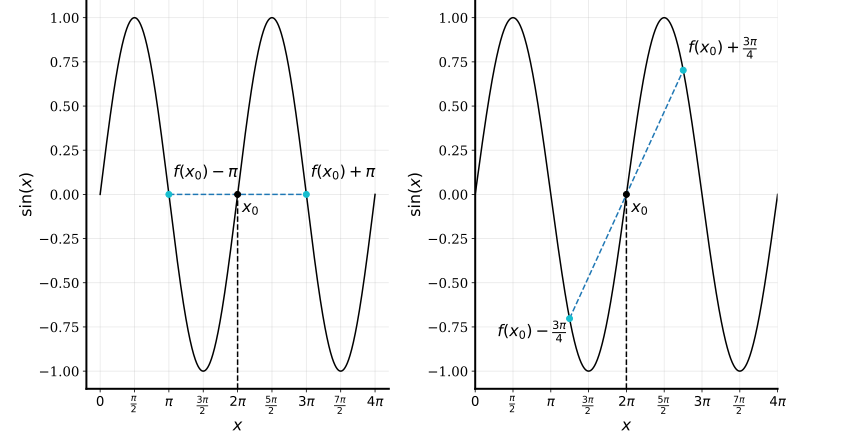
\includegraphics[width=\textwidth]{figures/central_periodic.pdf}
    \caption{Central difference approximation for the function $f(x) = \sin{x}$ using $h = \pi$ and $h = \frac{3 \pi}{4}$}
    \label{fig:central_periodic}
\end{figure}

\clearpage
\thispagestyle{plain}
\chapter{Framework and Partitioning Algorithms}\label{sec:framework}
This chapter introduces the framework that was implemented to generate workloads, partition data, and eventually benchmark a custom index that uses the partitioning. Note that the terms partitions and segments will be used interchangeably in the following.
\begin{figure}[H]
    \centering
    \includegraphics[width=\textwidth]{figures/pipeline.pdf}
    \caption{Framework Overview}
    \label{fig:framework}
\end{figure}

\section{Overview}
As we can see in \Cref{fig:framework}, the origin of all processes is the underlying data that we want to index and a query workload. However, we can also generate our own workloads through a Python script inside a Jupyter notebook. There, we can specify properties like the distribution and type of queries (point, range) that should be generated to access the data through the index. Because we wanted a fast workflow of generating and visualizing, we chose this approach. It has, however, the disadvantage that the workloads have to be saved to a file such that later on, the benchmarks can access them. Before they are saved, however, the queries generated in this step are divided into a train and test workload. The test workload will later be used in the C++ benchmarking.

Given the train workload, the partitioning algorithms that are described in \Cref{sec:frequency} and \Cref{sec:purity} can analyze the corresponding properties of the workload and will produce a partitioning of the underlying data. The resulting partitions are then saved to a file with additional information about each partition that can be used for the index construction. This information contains the relative frequency of a segment compared to the others and whether the segment mostly received point queries.
With these partitions, the index is bulkloaded from the data where each partition corresponds to an individual leaf node. The additional information is used to modify our index's structure and physical specialization. For example, if only point queries access a segment, it could be beneficial to manage data access through a hash table instead of a normal B-tree leaf. The next step is to execute the test workload on the index and compare it to other state-of-the-art indexes that were introduced in \Cref{sec:related_work}, namely a B$^+$-tree, an Adaptive Radix Tree (ART), and a Piecewise Geometric Model index (PGM).

\section{Workload Generation} \label{sec:wklgeneration}
The ultimate goal of this work is to generate a good partitioning for the index construction like it was mentioned in \Cref{bg:hybrid}. The inputs to the partitioning algorithms are, therefore, a dataset and a workload sample which we know is representative of the expected workload. However, to evaluate and test the algorithms and modifications, we required a flexible way to generate workload data, especially since it proved hard to find available real-world workload data. Although we do not have real-world workload data, we used our synthetic workload generation on real-world datasets in the hope that we get representative results. The workload generation is done in a Python script specifying a series of \verb|Region| objects. We have a basic repertoire of distributions (like uniform, zipfian, ...) that we append or overlap to create many different and more complex workloads. The \verb|Region| objects contain the following information:

\begin{itemize}
    \item \verb|index|: Whether the generation happens index-based or domain-based. Index-based means that we draw valid indices according to a distribution and then resolve the data values at these indices, domain-based means that we draw from the data domain, i.e.~we can draw values that fall inside the domain but are not present in the data itself. This cannot happen for an index-based generation.
    \item \verb|min, max|: The minimal and maximal values that indicate the region boundaries. In the index-based setting, these represent two indices that form the boundaries of this region. If we are in the domain-based setting, they represent the range of values from the data domain from which values can be generated.
    \item \verb|qtype|: The query type that should be generated in this region, e.g.~point or range queries
    \item \verb|num|: The number of queries in this region
    \item \verb|distribution|: The distribution underlying the generated queries in the region, e.g.~normal, uniform, ...
\end{itemize}

This gives us a very flexible way to generate arbitrary workloads. Note that while the partitions returned by our partitioning algorithms are mutually disjoint, the \verb|Region| objects used for workload generation do not need to be disjoint. This only means that we can overlap the boundaries of the objects to generate even more flexible workloads. In fact, it is the only way to generate regions of the data that are accessed through multiple types of queries, e.g.~through both point and range queries. 

As an example, \Cref{lst:generation} shows the code that would be used to generate a bimodal distribution of point queries. This is achieved by overlapping the two specified regions so that the two normal distributions form a bimodal distribution. The overlap is achieved by specifying the \verb|min| and \verb|max| attributes such that the \verb|max| of the first distribution is greater than the \verb|min| of the second distribution. In this case, the first normal distribution covers the first 70\% of the keys and the second distribution covers the last 70\% of the keys. 40\% of the keys in the middle will receive queries generated from both the first and the second distribution. The corresponding query distribution can be seen in \Cref{fig:bimodal}. Of course, the query distribution  depends on the data distribution it is applied to. While the data distribution in the first row was uniform to show the shape of the query distribution, the second row shows the same query distribution when sampling from exponentially distributed data.

\begin{lstlisting}[language=Python, caption=Example workload generation from Region objects, label=lst:generation]
    regions = [
        Region(
            qtype=QueryType.POINT, 
            num=100000, 
            distribution=DistributionType.NORMAL, 
            index=True, 
            min, max = 0, 0.7*len(data)
        ),
        Region(
            qtype=QueryType.POINT, 
            num=100000, 
            distribution=DistributionType.NORMAL, 
            index=True, 
            min, max =0.7*len(data), len(data)
        )
    ]
    wkl = Workload.from_regions(data, regions)
\end{lstlisting}

\begin{figure}
    \centering
    \includegraphics[width=\textwidth]{figures/bimodal.pdf}
    \caption[uniform and exponential query distributions after bimodal sampling]{CDF and query distribution of a bimodal workload on uniformly (top) and exponentially (bottom) distributed data}
    \label{fig:bimodal}
\end{figure}

After the queries are generated, we randomly sample a given fraction of them and remove these from the original queries. Similar to Machine Learning methods, we only use one of the resulting two sets to create our partitioning (training); the second set is later used for evaluation (testing) and immediately saved to a file. This ensures that we do not just design optimal partitions for the training queries. Instead, the partitions should be suitable for the underlying population of which train and test workload are only samples.

\section{Partitioning algorithms}
The next step in the framework is to use the train workload to find partitions in the data. There are many properties that one could look at when analyzing query workloads, but inspired by the works in \Cref{sec:related_work}, we decided to focus on two properties and look at how we could use these to partition the data and create segments: Frequency and Purity.

\subsection{Partitioning by Frequency} \label{sec:frequency}
The first algorithm analyzes the frequency of query accesses for each key in our dataset. The motivation behind using the frequency as a partition property is that, hopefully, we can benefit from caching effects during the execution of the test workload. We hope that the path to highly frequent segments remains in the cache so that subsequent queries can retrieve the location of the corresponding keys faster. On the other hand, the path to rarely touched segments should not be present in the cache most of the time. Additionally, by analyzing the frequency, we can use that information to change the structure of the index. The first idea in this regard would be to shift highly frequent segments higher up in the tree, to prevent expensive pointer chasing when traversing the index.

We first realized that traversing our data key-by-key and comparing them with each other is not useful for a generalizing partitioning algorithm because we can only operate on a train workload that is sampled from the general workload distribution. If we used these key-by-key comparisons for the frequency to create partitions, we would probably overfit the patterns in the train workload, even though these might only be caused by noise and not be present in the general distribution. Therefore, we employ an approach that tries to maximize the previously mentioned goal: find partitions where keys are accessed roughly the same amount of times. Regions with almost no query accesses will be put in one partition, resulting in the segment not being loaded very often. On the other hand, regions with similarly frequent keys will result in the  corresponding segment remaining in the cache if the frequency is high enough. However, one downside to this approach is that segments could become very large. As all information about a partition is contained in a single leaf node, large segments will prevent them from being cached entirely, as they are simply too large to fit in the cache. Still, parts of the node may remain in the cache. Additionally, we can hope that the inner nodes on the path between the root node and this leaf node remain completely in the cache since their size is fixed.

As already described in \Cref{bg:numerical}, we want to use finite difference approximations to estimate the derivative of the frequency our keys are accessed. Since the key space is discrete, the frequency function is discrete, so using the finite difference approximations is appropriate. We designed a single-pass algorithm that tries to find plateaus in the workload distribution by calculating the average change in frequency over a sliding window. It uses three phases depending on where it currently is concerning a plateau, which is heavily inspired by the three different approximations. As we have mentioned before, we do not want to use key-by-key comparison, as this is very sensitive to outliers. However, our finite difference approximations would do this: For example, the forward approximation would compare the current frequency to the frequency of the key with distance $h$ away. Instead of doing this, we compare the current frequency to the average frequency of the keys from the current key up to $h$ keys further away. Averaging over all these keys will enable us to generalize better and avoid starting new segments at outliers. The three phases are therefore:

\begin{enumerate}
    \item[I.] Start calculating a discrete forward difference approximation. As only keys "in the future" are considered, this phase is predestined to find an incoming plateau by checking if the calculated slope is near zero.
    \item[II.] After such a plateau was found, we used the central difference approximation to establish the boundaries of the plateau. We use this approximation now, as it considers keys from before and after the current one. This should give a better estimation of when a plateau is ending.
    \item[III.] Once the central approximation indicates that a plateau is ending (with an approximation value further away from zero), we switch to calculating the backward finite difference approximation to ensure that we find the exact end point of the plateau. We only consider previous keys, as we now know that an end is coming, giving us the best chance to catch the key responsible for significantly changing the slope.
\end{enumerate}


\begin{algorithm}
\caption{Partition by Frequency}\label{algo:freq}
\begin{algorithmic}[1] 
    \Procedure{PartitionFrequency}{$data, w, \delta$}
    \State $idx \gets 0,$ \; $n \gets data.size$ \; $w' \gets \lfloor \frac{w}{2} \rfloor$
    \While{$idx < n - w$} \Comment{Start Phase I}
        \State $falseAlarm \gets \text{False}$
        \State $fwdSlope \gets$ \textsc{ForwardDiff}($data, idx, idx + w$)
        \If{$| fwdSlope | \leq \frac{\delta}{w}$} \Comment{Potential partition start}
            \State $potStart \gets idx$
            \State $idx \gets idx + 1$
            \For{$i \gets 1$ to  $ w'$} \Comment{Start Phase II}
                \State $centralSlope \gets$ \textsc{CentralDiff}($data, idx - i, idx + w'$)
                \If{$| centralSlope | > \frac{\delta}{w}$}
                    \State $falseAlarm \gets$ True \Comment{Enforce minimal partition size}
                \EndIf
                \State $idx \gets idx + 1$
            \EndFor
            \If{\textbf{not} $falseAlarm$} \Comment{Plateau large enough}
            \State \textsc{Append}($result, potStart$)
            \While{$idx < n - \lfloor \frac{w}{2} \rfloor$} \Comment{Continue Phase II}
                \State $centralSlope \gets$ \textsc{CentralDiff}($data, idx - w', idx + w'$)
                \If{$| centralSlope | > \frac{\delta}{w}$}
                    \State\textbf{break} \Comment{Near end of plateau, go to Phase III}
                \EndIf
                \State $idx \gets idx + 1$
            \EndWhile
            \While{$idx < n - w$} \Comment{Start Phase III}
                \State $bwdSlope \gets$ \textsc{BackwardDiff}($data, idx - w, idx$)
                \If{$| bwdSlope | > \frac{\delta}{w}$}
                    \State \textsc{Append}($result, idx$) \Comment{End of plateau found}
                    \State\textbf{break} \Comment{Back to Phase I}
                \EndIf
                \State $idx \gets idx + 1$
            \EndWhile
            \Else \Comment{Plateau was not large enough}
            \State $idx \gets potStart + 1$ \Comment{Start over at Phase I}
            \EndIf
        \Else
            \State $idx \gets idx + 1$ \Comment{No small forward approx., go to next key}
        \EndIf
    \EndWhile
    \State \textsc{Append}($result, n$) \Comment{Add last boundary to $result$}
    \State \textbf{return} $result$
    \EndProcedure
\end{algorithmic}
\end{algorithm}

These phases can be mapped to \Cref{algo:freq}. The input to this algorithm is the data we want to partition, a window size parameter $w$ for the sliding window, and $\delta$ to control the strictness of what is still considered a plateau. After initializing our variables at the start (line 2), we begin to go over our keys as long as we can compute a forward difference approximation (line 3). We compute the forward difference approximation as described above, and if we may have found a plateau, we start the second phase (lines 6-8). However, to ensure that not every time we encounter a zero forward difference approximation, we start a new partition, we require that for the next $\lfloor \frac{w}{2} \rfloor$ keys, the central approximation stays close to zero (lines 6-15). This value was chosen purely heuristically. The variable $falseAlarm$ keeps track of whether our potential plateau is large enough. If it is not, we go back to phase one, beginning one key after the previous potential start (lines 33-35). This approach will cause the partitions to be at least $\lfloor \frac{w}{2} \rfloor$ keys long. If all the central approximations were near zero, we append this partition to our result (line 17). Then, we continue to calculate the central difference approximation as long as we see near zero values. Should this no longer be the case, we change to phase three with the backward difference approximation (lines 18-24). As soon as this backward difference approximation also becomes deviates too much from zero, we determine that the plateau has ended and therefore start a new partition (lines 25-32). If we initially did not have a small enough forward approximation for our current index, we just start over with the next key (lines 36-38). In the end, we append the last index to our partitions, as our convention is that the index representing the partition is the last index of the partition (line 40).

\subsection{Partitioning by Purity} \label{sec:purity}
The second algorithm does not analyze the frequency of a key but the query types that access the key. This way, we can distinguish between keys that are not requested at all by queries, those that are only accessed by one single type (e.g.~point or range queries), and those that are accessed by different types (e.g.~accessed through point and range queries, each). The motivation behind this approach is that we can use this information to adapt our hybrid index structure such that the underlying data structure is optimized for certain sub-ranges. One optimization that comes to mind is using a hash table for a segment that is only accessed through point queries. One can benefit from the faster lookup time, while the disadvantage of hash tables, the unsortedness of the keys, has no impact because we know that we have no range queries that access this segment.

Like the frequency algorithm above, we ruled out the use of key-by-key comparisons because of the generalization problem. Instead, we used a rather simple algorithm that tries to find the boundaries where the query type changes. The goal here is to determine partitions with pure access patterns, so one partition should mostly contain one query type (or only mixed accesses). The algorithm is a single-pass over the data, where we again consider a sliding window around the currently selected key. For each key, we store the predominant query type in that window, and as soon as we have a different major query type than for the previous key, we begin a new partition. We opted to use this simpler approach here, as we look at the mode of the query types in a certain window. While outliers in the frequency domain have the potential to change the average frequency significantly, an outlier in the query type will not affect the mode. However, we note that while a single range query in a region with otherwise only point queries does not affect the mode, it could still incur a significant performance cost later on because a range query is more expensive to perform on e.g.~hash tables.

In \Cref{algo:purity} we initialize our index at the point $\lfloor \frac{w}{2} \rfloor$, as we want to be able to calculate the mode across one whole window, which automatically means that the first $\lfloor \frac{w}{2} \rfloor$ keys always belong to the same partition (lines 2-3). We then calculate the mode across the query types for this window and proceed with the next key (lines 5-6). While we can still create a full window, we calculate the mode for this window, and if it differs from the previous key's mode, we end our partition (lines 7-11). Lastly, we need to update the variable that holds the previous key's mode to the current one and proceed with the next key (lines 12-13). In the end, we append the last index to conclude the last partition, as per our convention mentioned before (line 15).

\begin{algorithm}
\caption{Partition by Purity}\label{algo:purity}
\begin{algorithmic}[1]
    \Procedure{PartitionPurity}{$data, w$}
    \State $w' \gets \lfloor \frac{w}{2} \rfloor$
    \State $idx \gets w'$
    \State $n \gets data.size$
    \State $lastMode \gets$ \textsc{CalculateMode}($data, idx - w', idx + w'$)
    \State $idx \gets idx + 1$
    \While{$idx < n - w'$}
        \State $curMode \gets$ \textsc{CalculateMode}($data, idx - w', idx + w'$)
        \If{$curMode \neq lastMode$}
            \State \textsc{Append}($result, idx$)
        \EndIf
        \State $lastMode \gets curMode$
        \State $idx \gets idx + 1$
    \EndWhile
    \State \textsc{Append}($result, n$)
    \State \textbf{return} $result$
    \EndProcedure
\end{algorithmic}
\end{algorithm}

\section{Index Bulkloading and Benchmarking}
To understand how we incorporate the partitioning information into our index, we need to cover the general structure of the hybrid index and how it is built and bulkloaded before being benchmarked. Additionally, we look at how the index is altered by the partition information.

\subsection{Structure of the index}
The general structure of our index is very similar to the indexing framework presented by \citeauthor{Dittrich2021} \cite{Dittrich2021}. Our index has the same internal structure as a B$^+$-tree, but we do not fix the size of the leaf nodes. Instead, each leaf is designed to represent exactly a partition produced by the partitioning algorithms from before. As described in \Cref{bg:hybrid}, we have the flexibility to choose the data layout and search strategy inside each node separately. The default search strategy for the internal nodes (to locate the next child) and the leaf nodes (to locate the final position) was chosen as binary search, as we deal only with sorted data in this work. This restriction was applied here because if we were to partition unsorted data and obtain some partitions, their ranges (minimum and maximal value inside partition) would certainly not be disjoint. However, this characterizes the routing inside a B$^+$-tree-like structure. As this requirement would not be satisfied, we could not use the described internal tree-like structure, and it is not immediately clear how the routing inside the index needs to be designed to support such partitions. Therefore, we did not look into the case of partitioning unsorted data.

\subsection{Choice of leaf data structure}
The first way of optimizing our index given the partition information is to change the leaf data structure that is used to map the keys of our dataset to their positions. The default choice of a binary search with a sorted layout is well suited for a general workload where we would anticipate range queries, as we only need a lower bound point query and an additional scan towards the upper bound to determine all keys that qualify for the query. This is a sensible default, but we choose to use a hash table instead for a point query-only segment. As mentioned before, we achieve a better lookup performance for point queries, and as there are (almost) no range queries in the segment, we do not need to support an efficient lookup for them. Should we encounter a range query in the test workload, we can still guarantee the correctness of the results by converting the range query to a series of point queries that can be executed on the hash table. While this optimization seems straightforward, we could also change the leaf data structure for other different scenarios, although that was not further explored in this work.

\subsection{Transforming leaf nodes} \label{sec:leaftransform}
The next way of optimizing the index is to utilize the frequency of the partitions that are generated more effectively. Apart from only creating the partitions, one could also consider improving access times for frequently visited segments. One way of doing so was presented in \Cref{sec:related_work}, where the authors adaptively classified nodes as hot or cold based on current and past access statistics. Then they either applied a performance-optimized or space-optimized encoding to these nodes, depending on the classification. In the framework presented in \Cref{bg:hybrid}, this would correspond to a node mutation, where compression would be chosen and applied. Another approach that we wanted to look into is moving the leaf segments with a relatively large frequency higher up in the tree, which would result in a shallower path to the corresponding segment in our index. We suspect that we could benefit from caching effects here, as there are fewer nodes above the leaf segment that need to remain in the cache for faster access. This approach can be seen in \Cref{fig:frequencybulkload}. The top half shows the resulting index after bulkloading the data points 1, 4, 7, ..., 27, 29, and 30. A standard bulkloading approach starts by constructing the leaf nodes and proceeds with constructing inner nodes in a bottom-up fashion. In our example, the bulkloading would collect the three left-most leaf nodes to construct the left inner node one level higher up. The remaining leaf nodes would then be put in a second inner node because the first one ran out of capacity. However, if we knew that the keys in the third leaf node are frequently requested, we could decide to push this leaf node to a higher index level as done in the bottom half. In our example, we treat our leaf node as if it was an inner node one level higher up. We then need to construct the other inner nodes for this level, but we cannot treat the remaining leaf nodes as if they were only one instance of the bulkloading. If we did this, the left inner node would fill up to capacity and include the leaf node with keys 19, 22, and 24. This would result in two inner nodes whose ranges are no longer disjoint because the left one would include keys from 1 to 24, while the middle one (our original leaf) has a range from 14 to 18. Therefore, we treat the leaf nodes left from our original one and right from it as separate sub-problems to the bulkloading. The resulting inner nodes can then be treated as siblings to our original leaf node, which ensures that ranges of nodes on the same level are disjoint. At this point, we need to note that while we describe this approach here, we did not have enough remaining time to implement it and use it in our experiments.

\begin{figure}
    \centering
    \includegraphics[width=\textwidth]{figures/frequency_bulkloading.png}
    \caption[Incorporating frequency information into index bulkloading]{Resulting index after standard bulkloading (top) and after bulkloading with additional frequency information (bottom)}
    \label{fig:frequencybulkload}
\end{figure}

\clearpage
\thispagestyle{plain}
\chapter{Evaluation}\label{sec:evaluation}

This chapter covers the experiments we conducted to understand our partitioning algorithms and then compare our partition-based index to state-of-the-art index structures. We will briefly go over the setup and the software parameters that were used for the experiments in \Cref{sec:setup}. Then we cover the datasets and workloads on which the experiments were evaluated in \Cref{sec:datasets}. Finally, we present the results of the partitioning algorithms and benchmarks in \Cref{sec:respartitions} and \Cref{sec:resperformance}.

\section{Setup}\label{sec:setup}
All benchmarking experiments were conducted on a machine with NUMA architecture and two \textit{Intel Xeon X5690} processors with a base frequency of 3.47 GHz and 190 GB of RAM. The operating system was \textit{Arch Linux} with a kernel version \textit{linux 5.18.12}. For the compilation of the benchmarking, we used \textit{clang++ 14.0.6} with the release optimization level 3 (using the \verb|-O3| flag).

The implementation for our B$^+$-tree is the \textsc{TLX btree\_map} for the TLX B-tree by \citeauthor{TLX} \cite{TLX}. The ART implementation is the \textsc{ARTPrimaryLB} from \citeauthor{sosd-vldb} \cite{sosd-vldb} because of its support for lower bound queries. Concerning the PGM index, we chose to use the standard variant provided by \citeauthor{Ferragina:2020pgm} \cite{Ferragina:2020pgm}, the \textsc{PGMIndex}. As index configuration parameters, we chose an inner slot size of 16 and a leaf slot size of 32 for the TLX B-tree. For our index, we chose the same inner slot size for a better comparison. Our index does not require a leaf slot size since we have variable-length leaf nodes where the size is determined by the partitioning algorithms. The error parameter of the PGM index was set to $\epsilon = 128$.

\section{Datasets and Workloads}\label{sec:datasets}

To evaluate our partitioning algorithms, we looked at a variety of datasets and workloads to get a good understanding of how our partitioning algorithms work in practice. As for the datasets, we used synthetic and real-world representatives first to see how the algorithms perform on pure datasets with a clear distribution and then see if the algorithms translate well to irregular patterns in real-world data. The following real-world datasets are taken from \citeauthor{Kipf2019} \cite{Kipf2019}. All datasets consist of 64-bit unsigned integers.

\Cref{fig:cdfs} shows the cumulative distribution function (CDF) of the keys in different datasets that were used throughout the experiments. In the top row, the left graph shows the CDF of dense, uniformly distributed keys from 0 to 100 million. Naturally, it corresponds to a simple linear function. The middle graph displays the same for the real-world \verb|osm| dataset. We can see that there are many keys located around $0.5 \cdot 10^{19}$ and $1.0 \cdot 10^{19}$, which corresponds to the jumps at these points in the CDF. The third CDF shows the distribution of the real-world \verb|fb| dataset. The particular shape of the CDF here is caused by large outliers in the key domain. In the second row, we see CDF of the real-world datasets \verb|books| and \verb|wiki|. \verb|osm| contains uniformly sampled OpenStreetMap locations represented by their Cell IDs, \verb|fb| is a version of a Facebook user ID dataset, \verb|books| is a dataset of book sale popularity, and \verb|wiki| contains Wikipedia article edit timestamps. Each of them consists of 200 million keys.

\begin{figure}
    \centering
    \includegraphics[width=\textwidth]{figures/cdfs.pdf}
    \caption{Cumulative distribution functions (CDF) of different datasets}
    \label{fig:cdfs}
\end{figure}

For the workloads, we proceed according to the generation described in \Cref{sec:wklgeneration}. Our workloads are generated using multiple \verb|Region| objects, where each can specify a distribution from which the queries should be sampled. For the sampling, we used \textit{Python 3.10.4} in combination with the \textit{scipy (1.7.3)} package. Before we describe the workloads in each experiment, we will now give a short overview of the fundamental distributions depicted in \Cref{fig:distributions}. 

The first distribution is a \verb|uniform| distribution. Its probability density function is given by

$$
f(x)=\begin{cases}
  \frac{1}{b - a} & \mathrm{for}\ a \le x \le b, \\[8pt]
  0 & \mathrm{for}\ x<a\ \mathrm{or}\ x>b
  \end{cases}
$$

\noindent The parameters $a$ and $b$ correspond to the region boundaries in our framework, which means that all the keys in a uniform region have the same probability of being sampled for our workload.

\noindent The second distribution is a \verb|normal| distribution, whose PDF is given by

$$
f(x) = \frac{1}{\sigma \sqrt{2 \pi}} \exp{(-\frac{1}{2}(\frac{x - \mu}{\sigma})^2)}
$$

\noindent The parameters $\mu$ and $\sigma$ regulate the location and scale of the PDF inside our region and represent the mean and standard deviation. The normal distribution is symmetric around $\mu$, which means that the keys around the center of the curve have the highest probability of being chosen for the workload, while the probabilities of the keys decrease symmetrically the further away they are from the center.

\noindent The third graph shows the PDF of a \verb|lognormal| distribution with its PDF used by \textit{scipy}

$$
f(x, s) = \frac{1}{s x \sqrt{2 \pi}} \exp{(-\frac{\ln{(x)}^2}{2 s^2})}
$$

\noindent According to their documentation, the location and scale parameters $\mu$ and $\sigma$ can be incorporated via the formula $f'(x, s, \mu, \sigma) = \frac{f((x - \mu)/ \sigma, s)}{\sigma}$. The parameter $s$ is also used influence the shape of the distribution. This distribution is highly skewed, which results in a non-symmetrical access pattern for the queries. 

\noindent Similarly, the last graph was created by a \verb|gamma| distribution. The \textit{scipy} documentation defines the PDF as 
$$
f(x, a) = \frac{x^{a - 1} e^{-x}}{\Gamma(a)}
$$

\noindent where we can again incorporate location and scale parameters $\mu$ and $\sigma$ using the conversion $f'(x, a, \mu, \sigma) = \frac{f((x - \mu)/ \sigma, a)}{\sigma}$. The parameter $a$ serves the purpose of changing the distributions shape. A gamma distribution is generally speaking very customizable when it comes to its shape, but for the sake of our purpose, we only choose the parameters such that we get a skewed distribution that is slightly less skewed than the lognormal distribution.

\begin{figure}
    \centering
    \includegraphics[width=\textwidth]{figures/distributions.pdf}
    \caption{Probability density functions (PDF) of different distributions}
    \label{fig:distributions}
\end{figure}

\section{Influence of Hyperparameters}\label{sec:respartitions}
Both our algorithms are based on a sliding window approach, so the hyperparameters to our partitioning naturally include the window size $w$. For the frequency approach, we also need to specify how lenient we want to be when determining whether a window is a plateau. As we will only seldom see that our frequency function is perfectly uniform in certain regions, we introduce the hyperparameter $\delta$. It gives us an upper bound for the absolute value of the discrete first-order derivative approximations over a window to allow classification as a plateau still. 

Although we have extensively varied these parameters throughout our experiments, we could not determine automatically what these parameters should be for a given dataset and workload. Only through manual inspection of the dataset and workload distribution could we choose an acceptable configuration such that the partitions intuitively fit the workload. This is easier for workload distributions like the uniform one, where we could directly adjust our window size $w$ and $\delta$ to translate the uniform region to a separate partition. However, for others, like the normal distribution, this is not as easy, as we cannot determine any obvious plateaus. Should we choose the parameters such that a region around the peak becomes its own partition? Should there be partitions around the tails of the distribution? What about the regions in between? These questions arise when there are no clear boundaries in our query distribution. Unfortunately, throughout our experiments, we could not find an answer that generalizes to all possible query distributions.

\subsection{Purity partitioning}
To showcase the behavior of the purity partitioning algorithm, we can look at the comparison depicted in \Cref{fig:purinfluence}. Both scenarios show the same query distribution, but on the left, we created partitions with the parameter $w = 200$, whereas on the right, we used $w = 1000$. The underlying data is a uniform, dense array of keys from 0 to 10,000. Over these 10,000 keys, we sampled uniformly 200,000 point queries each in the intervals [0, 3000) and [3300, 10000). In the remaining interval from [3000, 3300), we sampled uniformly 50,000 range queries. As the interval of range queries is only 300 keys long, the partitioning with $w = 1000$ will not recognize this region as a separate partition because at no point in this region will a sliding window of size 1000 produce a majority of range queries. Even in the middle of the range query region, at key 3150, the sliding window will only see 300 keys requested by range queries but 700 keys requested by point queries. Therefore, the whole key space is seen as a partition of mostly point queries. On the one hand, for $w = 200$, we can recognize that at key 3001, we have 99 point queries and 101 range queries in our window. Therefore, our algorithm will start a new partition at this index. On the other hand, as soon as we reach key 3301, we will see 99 range queries and 101 point queries, which will result in the start of yet another partition. As we can see, the window size selection plays a major role in whether regions of alternating query types can be identified. If we do not set this parameter appropriately, we might very well get subpar results for our partitioning.

\begin{figure}
    \centering
    \includegraphics[width=\textwidth]{figures/purity_influence.pdf}
    \caption[Influence of purity hyperparameter]{Influence of window size parameter $w$ on purity partitioning. Left shows $w = 200$, right shows $w = 1000$.}
    \label{fig:purinfluence}
\end{figure}

\subsection{Frequency partitioning}
For our frequency approach, we have two parameters that need to be chosen beforehand. The first is identical to the purity approach presented in the last section, the window size $w$. The different finite difference approximations are then calculated over the frequencies in this window. A perfectly uniform region in the frequency domain would result in an approximation of zero. However, in practice, we will most likely see more variance in the frequency and also noise that does not follow a general pattern. Therefore, we do not get an optimal approximation of exactly zero, but something in its near vicinity. The parameter $\delta$ then influences whether this deviation from zero is small enough for it to be negligible. As an example, a configuration of the algorithm with window size $w = 100$ and $\delta = 3$ will allow a deviation of $\frac{\delta}{w} = \frac{3}{100} = 0.03$. For the forward approximation, this means that the frequency of the current key $f$ at index $i$ and the average frequency of the next 100 keys can differ by 3. The corresponding maximal slope $s$ is then identical to the previously introduced fraction $\frac{\delta}{w}$:

$$
s = \frac{\Delta y}{\Delta x} = \frac{(f + 3) - f}{(i + 100) - i} = \frac{3}{100} = \frac{\delta}{w}
$$

\noindent This relation is visualized in \Cref{fig:freqinfluence}. For the sake of simplicity, the workload represents a function with the following definition:

$$
f(x)=\begin{cases}
  40 & \mathrm{for}\ 3000 \leq x \leq 4000, \\[8pt]
  10 & \mathrm{for}\ x<3000\ \mathrm{or}\ x>4000
  \end{cases}
$$

\noindent where $f(x)$ evaluates to the access frequency of key $x$.

\noindent Note that this workload was not sampled using our framework. While our framework is very well able to do this generation, it inherently incorporates some variation in the steps due to the random nature of sampling. To showcase the influence of the parameters $w$ and $\delta$ however, we want to have a static frequency across each step with no variation.

\begin{figure}
    \centering
    \includegraphics[width=\textwidth]{figures/freq_influence.pdf}
    \caption[Influence of frequency hyperparameters]{Influence of window size parameter $w$ and $\delta$ on frequency partitioning. The first row shows the influence of $\delta$ when the window size is fixed, and the second row shows the influence of $w$ when $\delta$ is fixed.}
    \label{fig:freqinfluence}
\end{figure}

The first two graphs show the influence of $\delta$ when the window size $w$ is fixed. For this we chose $w = 400$ and $\delta_1 = 29.99, \delta_2 = 30$. According to our algorithm, to conclude a partition, we need a point where the average frequency of the left 200 keys differs more than 29.99 (30) from the average frequency of the right 200 keys. If we now look at key 3000, we see that the left 200 keys have an average frequency of 10 and the right 200 keys have an average frequency of 40. The difference is therefore 30. As $30 > 29.99 = \delta_1$, our partitioning algorithm produces a new partition for the keys between 3000 and 4000. However, since 30 is not strictly greater than $\delta_2 = 30$, the algorithm produces no separate partition in the second case.

In the second row, we investigate the influence of $w$ when $\delta$ is fixed. We chose $\delta = 29.99$ and $w_1 = 2000, w_2 = 2002$. Again, to form a new partition, we need a point where the average frequency of the left 1000 (1001) keys differs more than 29.99 from the average frequency of the right 1000 (1001) keys. Let us now look again at key 3000. We can determine that the average frequency of the left 1000 and 1001 keys is 10. However, for the right keys, there is a difference. If we only look 1000 keys to the right, we exhaust the complete plateau of elevated frequencies. The average frequency is here 40. However, if we look 1001 keys to the right, we not only include all keys with frequency 40 but also one with frequency ten again. Therefore, the average frequency is $\frac{40 \cdot 1000 + 10}{1001} = 39.97$. The difference in average frequencies is 30 for the first case and 29.97 for the second. As our threshold is $\delta = 29.99$, the algorithm will only create a new partition in the first case, not in the second.


\section{Benchmarking results}\label{sec:resperformance}
After all indexes are constructed, we run the test workload ten times on each of them, shuffling after each run to prevent caching effects. We apply the same strategy as \citeauthor{Dittrich2021} when it comes to range queries, namely that they can be translated to a lower bound query and a subsequent scan of the data array. This is possible because our scenario is that index entries map keys to their position in a sorted array. The scan of the data array is independent of the index type and can be neglected. Furthermore, we remark that all lookup time charts have small black bars that indicate the standard deviation across ten runs. As these are barely noticeable, we conclude that our results are quite stable.

\subsection{Purity partitioning on sharp borders}
First of all, we conducted an experiment that was designed to confirm the results of \citeauthor{Dittrich2021} \cite[Optimized vs Heuristic Indexes]{Dittrich2021}. It serves to answer the question: 

\begin{center}
    \textit{Can we reproduce the results presented in their paper?}
\end{center}

\noindent While they handcrafted the boundaries, the partitions for the experiment here were generated by our purity partitioning algorithm. The workload that was executed on the data was split into three regions: the first 10 percent of the keys, the next 75 percent, and finally the remaining 15 percent. The first region received 20 percent of the total queries as point queries, the second region received 10 percent of the queries as point queries, and 20 percent as range queries. The final region received the remaining 50 percent of queries as point queries. For our experiment, we used 2 million queries in total of which 1 million served as a train workload and 1 million as a test workload. For the benchmarking on the test workload, we, therefore, had the queries depicted in \Cref{tab:poc_wkl}.

\begin{table}
\centering
\begin{tabular}{rrrrr}
\hline
Region & from & to   & number queries & query type \\ \hline
1      & 0    & 0.1  & 200k           & Point      \\
2      & 0.1  & 0.85 & 100k           & Point      \\
2      & 0.1  & 0.85 & 200k           & Range      \\
3      & 0.85 & 1    & 500k           & Point      \\ \hline
\end{tabular}
\caption{Query Distribution for our first experiment}
\label{tab:poc_wkl}
\end{table}

\begin{figure}
    \centering
    \includegraphics[width=\textwidth]{figures/exp1_query_dist.pdf}
    \caption[uniform, osm and books query distribution after sharp boundary sampling]{Query distribution in our first experiment, sampled over a uniform, dense dataset, the osm and the books dataset}
    \label{fig:poc_dist}
\end{figure}

The resulting query distribution, together with the boundaries that our algorithm produced, is visualized in \Cref{fig:poc_dist}. As we can already tell from the description of the query distribution, we have two very clear boundaries when looking at the purity. While the first and last regions are only requested by point queries, we can see that the middle part receives both types of queries. Notably, we see mostly orange and green bars in the figure in this region, as this range contains 150 million keys but receives only 300 thousand queries. While there is some overlap in these queries, it is rather unlikely that one key from this range is selected for both point and range queries. This overlap would result in a purple bar in the figure. Nevertheless, a generalizing partitioning algorithm should recognize the boundaries and create three partitions accordingly. 

The window size parameter $w$ was set to 10,000 because we know that the regions defined above contain multiple millions of keys. The resulting partitions reflect this anticipation. Only for the \verb|books| dataset do we see one additional partition in the middle of the mixed region. This extra partition is caused by the rare scenario we just described. While we have a region with mostly disjoint point and range queries, there are enough keys that are both requested by point and range queries. So our algorithm recognizes that the majority changes from range queries to mixed queries in our sliding window, creating this additional partition. We decided to include the same datasets here as \citeauthor{Dittrich2021}, but we also evaluated this workload on the remaining datasets \verb|fb| and \verb|wiki|. The corresponding plots can be found in \Cref{app:sharp}.

\Cref{fig:poc_times} shows the results of executing the test workload on the different data structures. AS we expect, our index consists of three leaf nodes, where the outermost contain a hast table and the middle one is a B-tree like leaf with sorted data. Depicted is the average lookup time for the 1 million queries. Across the three datasets, the TLX B-tree requires the most amount of time, between 700 and 800 ns. Both ART and PGM can outperform our index with lookup times around 120 ns for the uniform dense dataset. On the other two real-world datasets \verb|osm| and \verb|books|, our custom index achieves a competitive lookup time of around 250 ns, while ART and PGM require between 300 and 400 ns each. As \citeauthor{Dittrich2021} have also mentioned in their experiment, the uniform dense dataset is close to optimal for PGM and ART, which inherently puts our index at a disadvantage.  

\begin{figure}
    \centering
    \includegraphics[width=0.9\textwidth]{figures/poc_times.pdf}
    \caption[uniform, osm and books lookup performance after sharp boundary sampling]{Average query lookup time on uniform, dense data, and the osm and books dataset}
    \label{fig:poc_times}
\end{figure}

To come back to our initial question, we conclude that when there are optimal preconditions (i.e.~sharp transitions between query types), it is indeed possible for our partitioning algorithms to produce partitions that can compete with the state-of-the-art indexes ART and PGM. However, this custom workload is very customized to create a best-case scenario for our algorithm, with clear boundaries between point and range queries. The next experiments will cover our partitioning algorithm's performance in less optimal but more realistic scenarios.

\subsection{Worst case considerations}
Following the previous optimal setting, we looked at scenarios that are the worst case for our partitioning algorithms. The question that we want to answer through this experiment is:

\begin{center}
    \textit{What is the performance of our workload-based partitioning in the worst case?}
\end{center}

\noindent We first look at the scenario that represents the worst case for our frequency algorithm. The first graph in \Cref{fig:freqworst} shows the uniform query distribution across a uniform dataset with 10 million keys. Since we have no variation across the whole dataset, our partitioning algorithm generates only one large partition. To achieve this result, a window size of $w = 200$ and $\delta = 1$ was already sufficient. We have decided to look at two extremes as the worst case for the purity algorithm. Here, 2 million point and range queries are distributed uniformly across the same uniform dense dataset. The first case uses a large window with window size $w = 1000$. This window is large enough to neglect the variation between keys that are requested by point and/or range queries. The second case happens when we choose a smaller window size of $w = 200$. Here, the sampling variance is large enough to continuously cause the algorithm to start new partitions because the majority of query type changes in the sliding window. Instead of one partition, we end here with nearly 10,000 partitions. That is why the third graph is seemingly completely red. There are just too many partitions to see the space in between. Notice that we reduced the dataset size from 100 million to 10 million points. This is due to the implementation of our frequency algorithm in \textit{Python}, which already took several minutes to run on the reduced dataset. While there are ways to optimize the run time, e.g.~not computing the mean of the window for every step of the sliding, instead keeping track of the contents of the window and only adding/removing at the start/end, we only found time to include this optimization in the simpler purity algorithm. 

\begin{figure}
    \centering
    \includegraphics[width=\textwidth]{figures/exp3_query_dist.pdf}
    \caption[Worst case query distributions for partitioning]{Query distribution in the worst case for frequency partitioning}
    \label{fig:freqworst}
\end{figure}

The results of this experiment can be seen in \Cref{fig:freqworsttimes}. While our baseline B-tree index needs around 500 ns for one lookup, ART and PGM achieve significantly better lookup times below 200 ns. As mentioned before, uniform dense data is almost the best case for these index structures. Our index performs significantly worse than these two but is still competitive with the B-tree. We also notice that one single partition is not really the worst case, as our index needs around 350 ns per query. The performance is worse when we have many small partitions, i.e.~for the purity algorithm with a small window size. Here our index needs approximately the same time as the B-tree.

Returning to our initial question, we can conclude that in the worst case, the performance of our index degrades significantly. While the wrong choice of hyperparameters can lead to only one single partition or a multitude of small partitions, we found that our index with one single partition still performs better than the index with lots of partitions. Although the results suggest that our index stays competitive with a B-tree, we need to consider the extra time the partitioning takes. Including this, we would rather choose a B-tree over our index when the lookup times are only similar. We need to note, however that we described a possible optimization depending on the frequency information in \Cref{sec:leaftransform}, which, as mentioned, was not implemented yet. Therefore, the results here might be improvable if this or a comparable technique were realized. 


\begin{figure}
    \centering
    \includegraphics[width=0.9\textwidth]{figures/exp3_poc_times.pdf}
    \caption[Worst case lookup performance for partitioning]{Average query lookup time on a uniform, dense data using worst-case workloads}
    \label{fig:freqworsttimes}
\end{figure}

\subsection{Frequency partitioning over skewed distributions}
The next question that we considered was whether our index performed well under more realistic query distributions. According to \citeauthor{Anneser2022} \cite{Anneser2022}, common patterns in real-world workloads often include skewness. This experiment, therefore, answers the question:

\begin{center}
    \textit{Can our workload-based partitioning yield a comparable performance to the state-of-the-art under skewed workload conditions?}
\end{center}


\begin{figure}[!ht]
    \centering
    \includegraphics[width=0.9\textwidth]{figures/exp2_query_dist.pdf}
    \caption[uni and osm query distributions after normal and lognormal sampling]{Query distribution using normal and lognormal workloads on a uniform dense and the osm dataset}
    \label{fig:skeweddist}
\end{figure}

\noindent Similar to their workload selection, we also included a normal and lognormal workload to answer this question. As a third skewed workload, we included a gamma distribution. The parameters for the normal and lognormal distribution were selected according to \citeauthor{Anneser2022}. For the normal distribution, we choose $\mu = 0.5, \sigma = 0.03$, for the lognormal distribution, we choose $s = 0.7, \mu = 0, \sigma = 0.1$ and for the gamma distribution, we choose $a = 1.2, \mu = 0, \sigma = 0.1$. As the gamma distribution is very similar to the lognormal distribution with just slightly less skewness, we include all relevant plots in \Cref{app:skew}. We choose to evaluate the distributions on uniform, dense data and the real-world \verb|osm| dataset because it has different patterns across the dataset. The other real-world datasets mostly have only one significant distribution pattern, and as the partitioning algorithm takes quite some time to run, we decided not to investigate them further. For the same reason, we again decided to choose the reduced datasets with a size of 10 million. 

\Cref{fig:skeweddist} shows the query distribution of these workloads on the uniform dense and \verb|osm| dataset. For the \verb|osm| dataset, we can clearly see that the queries are mostly centered around the points where the dataset is especially concentrated. This relation is obvious when we look back at \Cref{fig:cdfs}. Because of the skewness, the lognormal distribution selects keys near the first jump in the CDF, whereas the normal distribution selects those near the second jump in the CDF. We tried to adjust the hyperparameter such that we do not fall into a case described in the previous experiment, namely a single large partition or thousands of small ones. In the end, we landed at window size $w = 200$ and $\delta = 0.15$, resulting in 60 to 116 partitions depending on the dataset and workload. Even small changes in both parameters resulted in situations like the worst cases from above. Because we do not have an automatic way to choose the parameters, we settled for the ones we found well aware that there might be a better configuration that we just did not try out.

\begin{figure}[!ht]
    \centering
    \includegraphics[width=0.9\textwidth]{figures/exp2_times.pdf}
    \caption[uni and osm lookup performance after normal and lognormal sampling]{Average query lookup time on uniform, dense data and the osm dataset using skewed workloads}
    \label{fig:skewedtimes}
\end{figure}


\Cref{fig:skewedtimes} shows the results of this experiment. We can directly see that there is a general trend across all scenarios, namely that the lognormal workload is faster to execute than the normal one. We can further observe that, especially for the uniform dense case, our index is significantly slower than ART and PGM, which take less than 100 ns. However, this difference is less significant for the osm dataset because ART and PGM need slightly more time per query. We can also observe that our performance is stable across the two different datasets, where we need around 350 ns for the normal workload and 250 ns for the lognormal workload.

Coming back to our question in the beginning, we need to state that our partitioning-based index is not competitive with the state-of-the-art index structures ART and PGM, at least when no optimization is performed based on the frequency. We also note that we can still outperform the B-tree, our weakest baseline.



\subsection{Influence of index misses}

\begin{minipage}{\textwidth}
As we have only sampled index-based until this point, the following question arises:

\begin{center}
    \textit{Does the number of queries requesting a key not in our index influence the performance of our index?}
\end{center}

\end{minipage}

\noindent To answer this question, we revisit the distributions from the previous experiment and see how our index performance changes when we do not completely sample index-based. To reiterate, index-based sampling means that we sample the indices of our underlying data and then convert these indices back to actual data points. This means that we will always sample a key that is present in our data. The second approach is sampling domain-based, meaning we directly select keys that fall in the range of our data points. For the sparse \verb|osm| dataset, this means that almost all keys that we sample domain-based will not be contained in the dataset itself, especially if we only use the downsampled \verb|osm| dataset with 10 million points. For our experiment, we chose to sample the \verb|osm| dataset with varying amounts of domain-based queries. We used uniform, normal and lognormal distributions with 0 \%, 20 \%, and 50 \% domain-based queries. We tried again to keep the number of partitions approximately equal across the different percentages, as we did not want to incur more costs by having to traverse more levels in our index. The configuration of hyperparameters for each combination of workload and percentage can be found in \Cref{tab:indexmisses}. As the query distributions on the \verb|osm| dataset are known from the previous experiment, we do not show them again here. The corresponding plots with small differences due to the new sampling method can be found in \Cref{app:misses}.

\begin{table}[ht]
\centering
\begin{tabular}{rrrrr}
\hline
distribution & percentage misses & $w$   & $\delta$ & partitions \\ \hline
uniform      & 20                & 200  & 0.12      & 29         \\
uniform      & 0                 & 200  & 0.13      & 21         \\
uniform      & 50                & 200  & 0.09      & 49         \\
normal       & 0                 & 500  & 0.15      & 85         \\
normal       & 20                & 200  & 0.15      & 83         \\
normal       & 50                & 200  & 0.15      & 148        \\
lognormal    & 0                 & 200  & 0.15      & 100        \\
lognormal    & 20                & 200  & 0.15      & 133        \\
lognormal    & 50                & 200  & 0.12      & 168        \\ \hline
\end{tabular}
\caption{Hyperparameter configuration depending on the workload distribution and the percentage of index misses/domain-based queries}
\label{tab:indexmisses}
\end{table}

\Cref{fig:exp4times} shows the results of this experiment. The first thing we observe is that the general trend from the previous experiment is also present here: the lognormal workload requires less time than the normal one. Another trend is that the more domain-based queries we have, the less time per query is required by all index structures. For the normal and lognormal workload distributions, there is almost no decrease in lookup time when going from 0 \% to 20 \%, which is very similar to all other indexes. The next step from 20 \% to 50 \% is connected to a decrease by 40 to 50 ns, which also happens for the other indexes. Only for the uniform sampling do we see a decrease of 100 ns when going from 20 \% to 50 \%. ART and PGM only decrease by approximately 40 ns in comparison. On the other hand, the B-tree also has a relatively large reduction of around 80 ns.

To summarize, we can say that the number of domain-based queries and, therefore, on our sparse dataset, the number of index misses impacts the average lookup time. An increase in this number for all indexes results in a decrease in the average query lookup time. Notably, our index does not seem to be an outlier to this general trend, the decrease we observe is always very similar to one of the other indexes.

\begin{figure}
    \centering
    \includegraphics[width=\textwidth]{figures/exp4_times.pdf}
    \caption[osm lookup performance after sampling with index misses]{Average query lookup time on the osm dataset, depending on the percentage of index misses}
    \label{fig:exp4times}
\end{figure}

\subsection{Discussion}
At last, we want to address some points that influenced our research when answering our questions. First of all, we had the goal of covering a wide variety of workloads which we tried to do with customized scenarios. However, as we mentioned before, it was very time-consuming to calculate and manually inspect the partitions in relation to the workload distribution. As we do not have a mechanism to adjust our hyperparameters $w$ and $\delta$ automatically, we had to iterate over these values until we found a reasonable configuration. This excludes those configurations that produce way too many or one single partition, as we have seen in our second experiment. Because this iteration includes the partitioning step that takes several minutes to complete, we focused on rather simple workloads with a reduced dataset size. We are well aware that reducing the real-world datasets from 200 million keys to 10 million is a step that threatens the generalizability of the results we found. 

Another point we would like to mention is the structure of our index. While the main goal of this thesis was to develop the algorithms for partitioning, we naturally needed a way to evaluate these. Apart from the visual inspection of created partitions, this was done using the indexing framework introduced in \cite{Dittrich2021}. While we managed to incorporate the purity properties into the index by changing the leaf data structures, we did not have enough time to also do this in the way it was described in \Cref{sec:leaftransform}. This is mainly due to the initial approach we targeted, namely moving leaves higher up in the index after it was created. This was not as straightforward as we initially expected because moving leaf nodes could result in necessary changes to the whole index. It might not be possible to just add a pointer to the child in an inner node one level higher up because all inner nodes operate at maximum capacity. In this case, we would need to split one inner node, rearrange the child nodes and add the new nodes to their respective parent nodes. If their parents also operated at maximum capacity, they would again need to split, which in the worst case leads to a cascade of changes throughout the index. However, for our purposes, we could directly rearrange leaves at the construction time of the index, which is the easier approach. An implementation there can be realized much quicker, but because we were too invested in the more complex approach, we did not think of the easier solution in time to incorporate it into our experiments. Also, because the frequency algorithm was the more sophisticated one, we used more experiments to evaluate it, but in the end, the results suffer from the fact that the frequency information inside a partition is not structurally exploited by the index. We hope that a corresponding enhancement will result in a better performance. As of now, our index is essentially just a B-tree with variable length leaf nodes, which does not provide a competitive lookup performance apart from very specialized scenarios. 



\cleardoublepage
\chapter{Conclusion and Future Work}

\begin{itemize}
    \item Previous results reproducable?
    \item What have we found?
    \item Does partitioning yield better lookup times?
    \item Is it beneficial to move leaves higher up in tree?
    \item Is it beneficial to use hybrid index structures (i.e.~change layout/data structure in nodes)
    \item Best case/worst case considerations?
    \item Future Work: Combination of metrics
    \item Future Work: Look at more data structures other than BinarySearchLeaves and Hashtables
    \item Future Work: What other workload metrics can be used for partitioning?
\end{itemize}

%=======================================================================================================================

\cleardoublepage
\printbibliography

\cleardoublepage
\setcounter{page}{1}
\pagenumbering{roman}
\begin{appendix}
    \chapter{Appendix}

%\section{Contents of the accompanying cloud storage}

\section{Additional plots for sharp borders experiment}\label{app:sharp}
In this section, we include the additional plots that were created for our first experiment with sharp region borders in the workload. \par 

\Cref{fig:app_exp1_query_dist} shows the query distributions that are created by our workload generation. \verb|fb| on the left presents the challenge that almost all keys are concentrated at the beginning of the dataset due to very large outliers. Therefore, our plot only shows a single bar representing most of the one million queries. For the wiki dataset on the right, we needed to increase our window size to $w = 20000$ to get our desired partitions; with $w = 10000$, our algorithm produced around 50 partitions.

\Cref{fig:app_exp1_poc_times} displays the average lookup times we obtained. Notice that the PGM index threw an exception during execution for the \verb|fb| dataset, which is why we do not have a data point there. We observe similar results to the three datasets presented in the main part of this work, with our index achieving around 250 ns as the average lookup time. We also note that the ART index can outperform our index on the \verb|wiki| dataset and achieves a comparable time to its performance on uniform dense data.


\begin{figure}
    \centering
    \includegraphics[width=\textwidth]{figures/app_exp1_query_dist.pdf}
    \caption[fb and wiki query distribution after sharp boundary sampling]{Query distribution for the workloads used in our first experiment. The queries were sampled on the real-world datasets fb and wiki with 200 million keys each.}
    \label{fig:app_exp1_query_dist}
\end{figure}

\begin{figure}
    \centering
    \includegraphics[width=\textwidth]{figures/app_exp1_poc_times.pdf}
    \caption[fb and wiki lookup performance after sharp boundary sampling]{Average query lookup time on the real-world datasets fb and wiki for our first experiment. The average is taken over one million queries.}
    \label{fig:app_exp1_poc_times}
\end{figure}

\clearpage
\section{Additional plots for skewed distributions experiment}\label{app:skew}
In this section, we include the additional plots that were created as part of the skewed workloads on a uniform dense and the osm dataset. The plots show sampling using a gamma distribution, which was very similar to the lognormal one we already used in the evaluation section. \par

\Cref{fig:app_exp2_query_dist} and \Cref{fig:app_exp2_poc_times} show the results. As we suspected, they are very similar to the ones we obtained from the lognormal sampling previously.

\begin{figure}[ht]
    \centering
    \includegraphics[width=0.75\textwidth]{figures/app_exp2_query_dist.pdf}
    \caption[uniform and osm query distributions after gamma sampling]{Query distribution for the gamma distributed workload. The queries were sampled on a uniform, dense dataset with 10 million keys, and the real-world dataset osm, downsampled to 10 million keys.}
    \label{fig:app_exp2_query_dist}
\end{figure}

\begin{figure}[ht]
    \centering
    \includegraphics[width=0.75\textwidth]{figures/app_exp2_poc_times.pdf}
    \caption[uniform and osm lookup performance after gamma sampling]{Average query lookup time on a uniform, dense dataset with 10 million keys and the real-world dataset osm, downsampled to 10 million keys. The average is taken over one million queries.}
    \label{fig:app_exp2_poc_times}
\end{figure}


\section{Additional plots for index misses experiment}\label{app:misses}
This section includes the additional plots that show the workload distribution when we sample index-based and domain-based. Because the underlying \verb|osm| dataset is very sparse, the percentage of domain-based queries is very close to the percentage of index misses because the sampled queries are most likely not present in our data. \par

\Cref{fig:app_exp4_uni_query_dist}, \Cref{fig:app_exp4_normal_query_dist} and \Cref{fig:app_exp4_lognormal_query_dist} show the results. We observe that for an increasing amount of domain-based queries, the overall query distribution slowly transforms into a distribution that resembles sampling index-based on a uniform, dense dataset. This is simply since we indeed sample queries in the range of the minimal and maximal value in the data. The range is just the interval [min, max] and can therefore be seen as a uniform, dense dataset over which we sample.

\vfill
\begin{figure}[hb]
    \centering
    \includegraphics[width=\textwidth]{figures/app_exp4_uni_query_dist.pdf}
    \caption[osm query distribution after uniform sampling with index misses]{Query distribution for a uniform workload. The queries were sampled on the real-world dataset osm with 10 million keys. The first graph shows the distribution for no index misses, the second for 20 \% index misses and the third one for 50 \% index misses.}
    \label{fig:app_exp4_uni_query_dist}
\end{figure}
\vfill

\begin{figure}[ht]
    \centering
    \includegraphics[width=\textwidth]{figures/app_exp4_normal_query_dist.pdf}
    \caption[osm query distribution after normal sampling with index misses]{Query distribution for a normal workload. The queries were sampled on the real-world dataset osm with 10 million keys. The first graph shows the distribution for no index misses, the second for 20 \% index misses and the third one for 50 \% index misses.}
    \label{fig:app_exp4_normal_query_dist}
\end{figure}

\begin{figure}[ht]
    \centering
    \includegraphics[width=\textwidth]{figures/app_exp4_lognormal_query_dist.pdf}
    \caption[osm query distribution after lognormal sampling with index misses]{Query distribution for a lognormal workload. The queries were sampled on the real-world dataset osm with 10 million keys. The first graph shows the distribution for no index misses, the second for 20 \% index misses and the third one for 50 \% index misses.}
    \label{fig:app_exp4_lognormal_query_dist}
\end{figure}
\end{appendix}

\end{document}
